%%This is a very basic article template.
%%There is just one section and two subsections.
\documentclass[a4paper]{article}
\usepackage{amssymb}
\usepackage{amsmath}
\usepackage{graphicx}
\usepackage{subfigure}

\begin{document}
	\begin{titlepage}
	
	\centering
	
	{\huge\bfseries Management Dashboard with IBM Cognos\par}
	\vspace{2cm}
	
	
	\begin{figure}
    \subfigure{
\includegraphics[width=0.25\textwidth]{FH}\par\vspace{1cm}}
    \hspace{5cm}
    \subfigure{
\includegraphics[width=0.25\textwidth]{KABEG}\par\vspace{1cm}}
	\end{figure}
	\vspace{1.5cm}
	
	{\Large\itshape Christopher Schmidt and Fabian Matschitsch\par}
	\vfill
	supervised by\par
	Dr.~Florian Hollomey
	\vfill
	{\large \today\par}	
	
	\end{titlepage}

	\tableofcontents
	\newpage

	\section{Introduction}
	Hier wird die Einführung stehen.
	\newpage
	
	\section{Hospital Information Communication}
	\subsection{General Communication}
		The general communication for hospital informations is about data of patients,
		medical results, laboratory results, radiographs, financial data, insurance
		data and much more. In the middle of the whole communication will be the
		Hospital Information System (HIS). This system stores the patient information
		and send this data to all other so called Subsystems. A Subsystem will be
		every system which get data from HIS. This systems can also send data back to
		the HIS. For all this communication between the systems there will be a
		standardized protocoll named Health Line 7 (HL7).\\
		The following systems could be subsystems of the Hospital Information System:
		\begin{itemize}
	    	\item Laboratory Information System (LIS)
	    	\item Electronic Medical Record (EMR)
	    	\item Pharmacy Management (PM)
	    	\item Insurance Management (IM)
	    	\item Financial System (FS)
	    	\item Radiology Information System (RIS)
	    	\item Appointment Management (AM)
	    	\item Emergency Management System (EMS)
	    \end{itemize}
	    \begin{figure}[!ht]
		  \centering
		      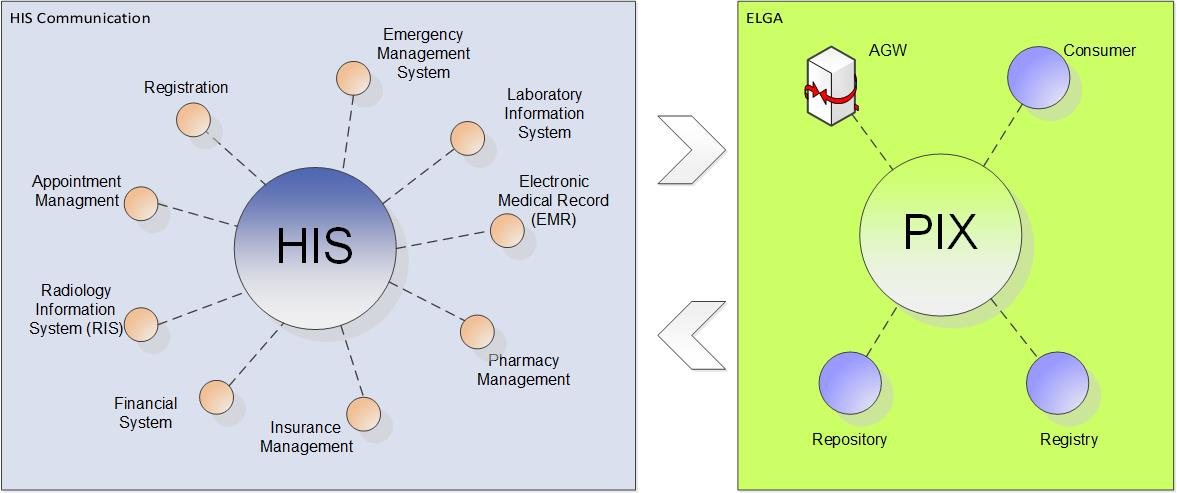
\includegraphics[width=1.0\textwidth]{HIS_Overview}
		  \caption{In the blue box on the left the Hospital Information System
		  Communication is shown. All this system communicate with the ELGA system
		  (on the right) which has an Patient Identifier Cross Referencing (PIX) and
		  an Access Gateway (AGW) for connecting and communicating with external
		  partners.}
		\end{figure}
	    Specially in Austria there will be new kind of system the so called ELGA.
	    This will give the posibility for people in Austria to have a look on their
	    own clinical record in digital way. The ELGA and the system of it will be
	    explained later on in chapter 4.\\
	    To get the systems speaking together a communcation server will be used.
	    This Server connects all the systems together and it is be able to make
	    mappings and database queries to get the right data in the right fields if
	    they are not.
	\subsection{Health Line 7}
		The Health Line 7 (HL7) is a standardized protocol in Version 2.5 and in
		future in Version 3 for the communication in eHealth systems. All systems
		who were communcating in an hospital will be called eHealth systems.\\
		HL7 provides a framework to exchange, integration, sharing and retrieval of
		electronix health information. It defines also the language, structure and the
		data types which are used for the communicatoin between the eHealth systems.\\
		The standard is human-readable and near to all eHealth systems are able to
		read data from HL7 and to export data in HL7.
		
	\newpage
	
	\section{IBM Cognos}
	\subsection{Introduction}
	Introduction to IBM Cognos
	\subsection{Framework Manager}
	Overview to Framework Manager
	\subsection{Report Studio}
	Overview to Report Studio
	\subsection{Data Topology}
	Overview to Data Topology build in Cognos
	
	\newpage
		
	\section{ELGA - Cross Document Sharing}
	\subsection{Weiß nicht genau?}
	\subsection{Next Steps}
	
	\newpage
	
	\section{Hospital Information System - AGFA Orbis}
	The Hospital Information System is the central system in inter-clinical
	communication. In this system all patient data will be stored and every booking
	and terms for the patients will be made.\\
	In the KABEG there are five hospitals and two different Hospital Information
	Systems. In future there should be only one HIS in the KABEG organisation. This
	HIS will be AGFA Orbis.
	\subsection{Orbis in the KABEG}
	At the moment 4 of 5 KABEG hospitals use AGFA Orbis as HIS. The main
	functionality of Orbis is to collect all patient data and sent it to all
	subsystems but Orbis has much more functionalities.\\
	Orbis consits of a lot of modules which were fit together to one system. One of
	this module is an appointment calender system. There the users can plan
	patients appointment but they can also use it as their own calender like an
	outlook calender. Another module is a module for planing and document
	surgeries. In this module the users have a view about all the operating rooms
	and see when the patients were coming in, when did the surgery starts or ends
	and much more.\\
	\begin{figure}[!ht]
		  \centering
		      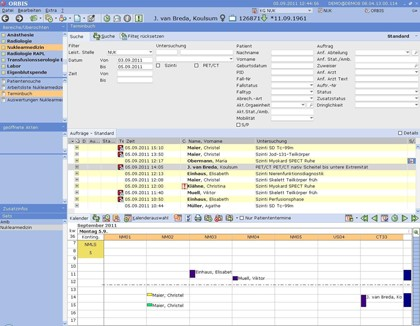
\includegraphics[width=0.6\textwidth]{orbis1}
		  \caption{Orbis Appointment calender system. There user can plan the
		  patients appointments and there own terms.}
	\end{figure}
	A third module is a planing module for orders of radiological
	examinations. There the users can order examinations and this will proceed an
	order on X-ray units and other devices. Also available in Orbis is a kind of
	overview about the clinical history for all the patients. There are
	stored values of laboratory investigations, links to medical reports which are stored
	in the Electronical Medical Record and much more.\\
	In many other Hospital Information Systems all the features above are not
	available and so for every little thing another subsystem will be used for.
	There will be a big advantage of Orbis. A big disadvantag on the other hand is
	that nearly all of these modules were productes of smaller companies which were
	regrated from AGFA. So many modules were migrated to Orbis and so it sometimes
	performe not as well as the users would like. This can be seen in the Orbis
	database which is described in the next chapter.\\
	\begin{figure}[!ht]
		  \centering
		      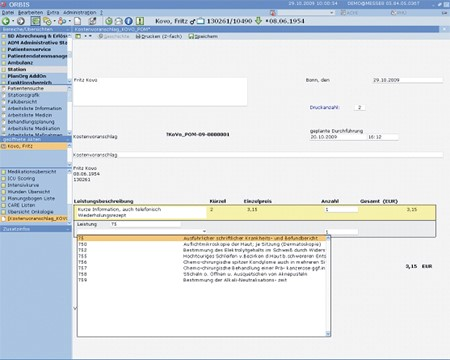
\includegraphics[width=0.6\textwidth]{orbis2}
		  \caption{Orbis Module for diagnosis and medical reports. There users can
		  select the diagnosis from a defined catalogue and write a free text to the
		  medical report which is stored as a PDF file in the Electronical Medical
		  Record.}
	\end{figure}
	\subsection{Orbis Database}
	The Orbis Database is grown over years. At the beginning it was a small
	Database for a small application to store patientdata. Because of many user
	wishes the company AGFA has to build in new features. \\
	\begin{figure}[!ht]
		  \centering
		      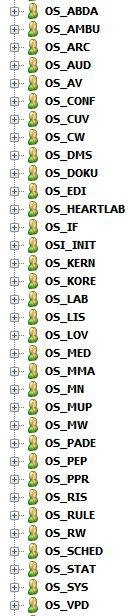
\includegraphics[width=0.12\textwidth]{orbis_db_schema}
		  \caption{Overview about the Orbis Database Schemas.}
	\end{figure}
	On one hand they develope some new features and modules for the application and
	on the second they buy some applications or the company which develope the application directly and
	merge them to Orbis. So the database became more and more schemas and tables
	and grew more and more. The main goal is to get a good performance for the
	user.
	\subsection{Actual Problems}
	The actual problem is that many database models were merged together. Many of
	them are not state of the art. So there are really big Database tables with
	many columns and without primary keys. They also don't have foreign keys to
	other other necessary tables. So sometimes it is not easy to get the right
	value to make a join over different tables.\\
	Another problem is get an overview about this Database also because of the
	problem descriped above. So if it is necessary to get simple values
	which are displyed in the application as well, the need arises to get really
	depth to the database. So it is not easy to get performant and correct
	asserting from Orbis.
	\subsection{Reports for Orbis}
	It was a goal of the project to build reports for boards of directors of the
	Orbis database in IBM Cognos. 
	\subsubsection{Overview about the reports}
	A Cognos Cube was build with AGFA and an automatically server job was develope
	to get actual data from the Orbis Database to this Cognos Cube.\\
	The next step was to use the IBM Cognos Report Studio to develope reports for
	the Web-Browser in HTML and for the iPhone application.
	\begin{figure}[!ht]
		  \centering
		      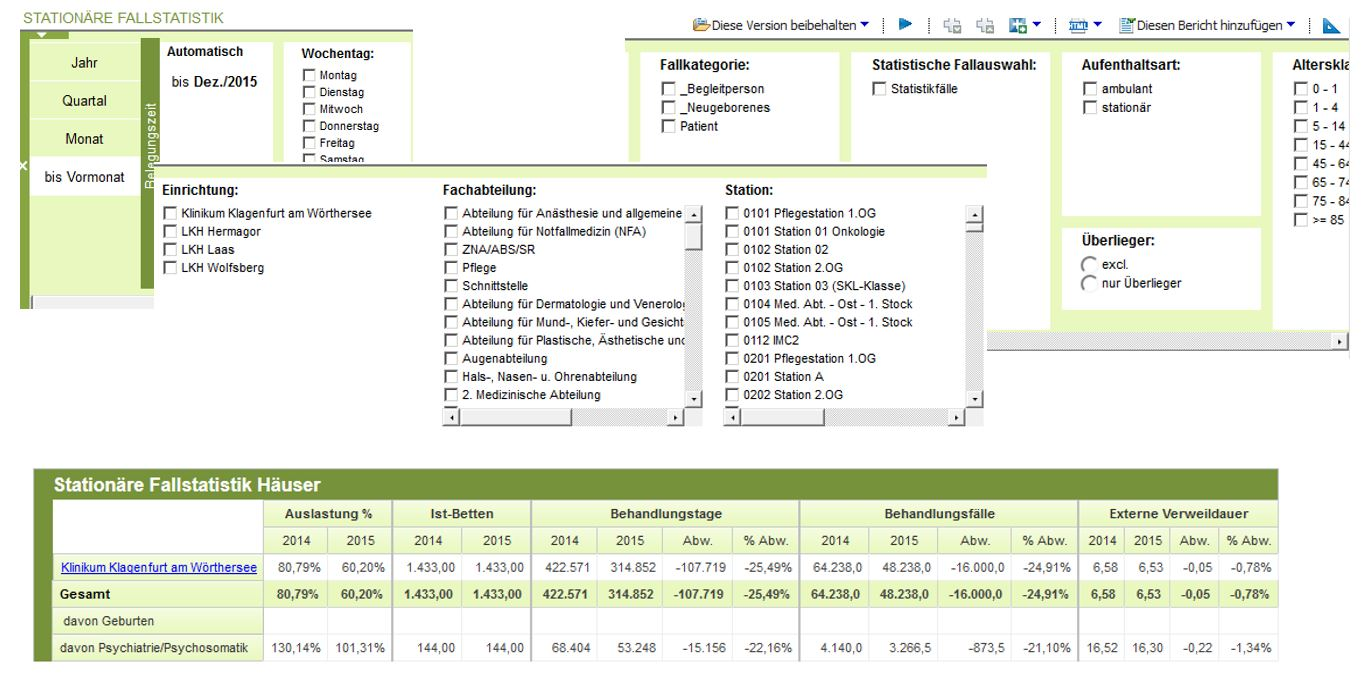
\includegraphics[width=1.0\textwidth]{reports_overview}
		  \caption{A view screenshots and overview about one of the reports. So it is
		  possible to select the hospital, department and station and so on. It is
		  also important to get a selection about in- or out-patient and the
		  timeline and much more other properties. The board of directors will get an
		  overview about the statistics they want and can select the properties on
		  their own.}
	\end{figure}
	\subsubsection{Result of the report}
	The results of the reports, which the boards of directors will get from it
	where displayed in tables, charts and diagrams. So it will esay for them to
	present statistical key figueres from the Hospital Information System and the
	billing and other statistics.
	\begin{figure}[!ht]
		  \centering
		      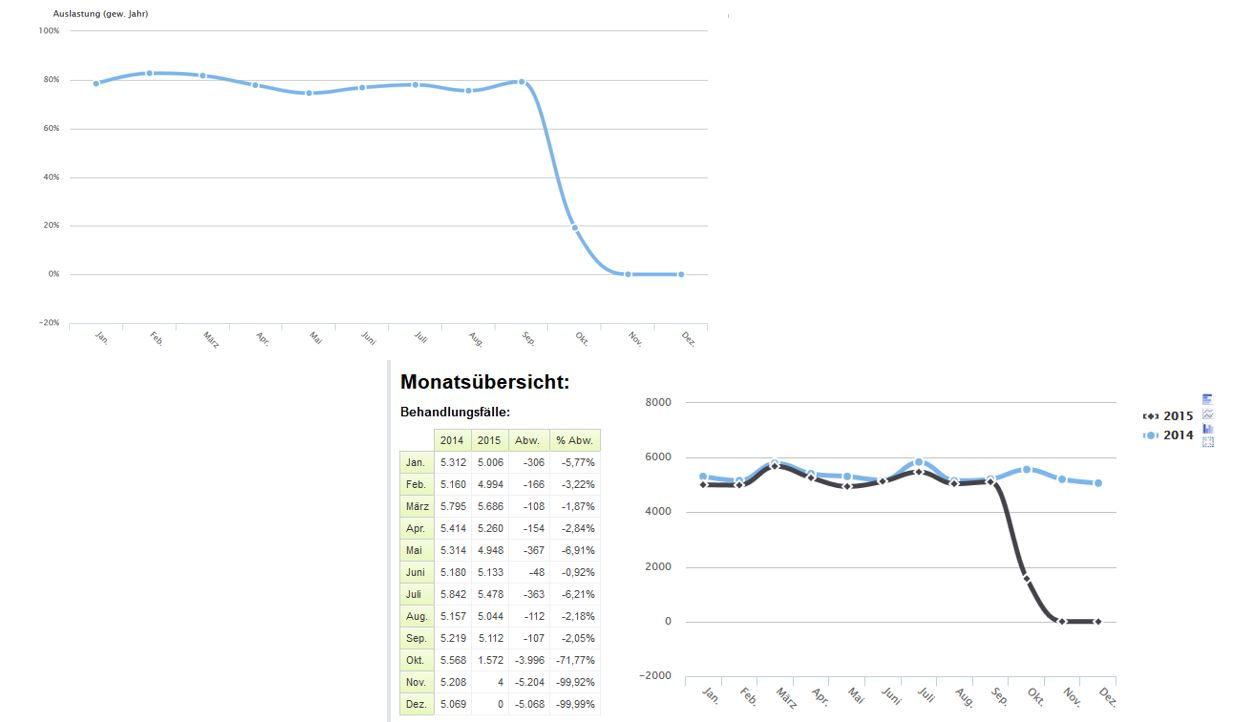
\includegraphics[width=1.0\textwidth]{reports_results}
		  \caption{An Example for a report for the in-patient statistic of the
		  Klinikum Klagenfurt. The load factor of the Klinikum is shown. It is
		  obvious the curve decreases to Zero on October. This is because the data
		  which were displayed for this tests are available ot October in the Cognos
		  Cube.}
	\end{figure}

\end{document}
